\documentclass[aspectratio=169]{beamer}
\usetheme{SimplePlus}

\usepackage{tikz}
\usepackage{pgfplots}
\usepackage{amsmath}
\usepackage{amssymb}
\usepackage{bm}
\usepackage{mathtools}
\usepackage{algpseudocode}
\DeclareMathOperator{\grad}{\nabla}
\renewcommand{\P}{\mathbb{P}}
\newcommand{\R}{\mathbb{R}}

\title[Finite Elements I]{The Finite Element Method II}
\author{Nicol\'as A. Barnafi}
\date{\today}

\begin{document}

\begin{frame}
    \titlepage
\end{frame}

\begin{frame}{Outline}
    \tableofcontents
\end{frame}

\section{2D Meshes and Shape Functions}

\begin{frame}{Meshes}
    \begin{columns}
        \begin{column}{0.6\textwidth}
            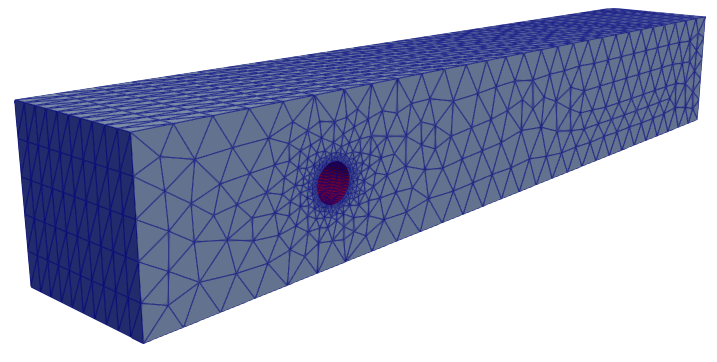
\includegraphics[width=\textwidth]{cylinder.png}
        \end{column}
        \begin{column}{0.35\textwidth}
            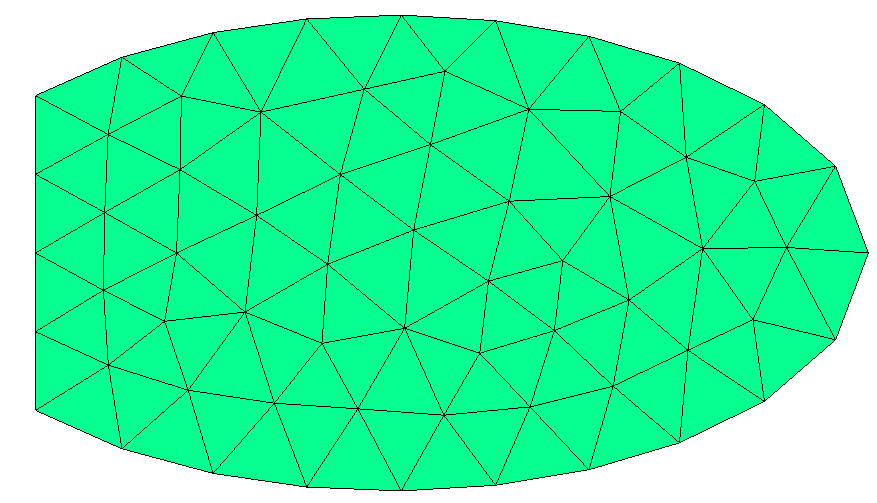
\includegraphics[width=\textwidth]{leaf.png}
        \end{column}
    \end{columns}
    Generating meshes is a \emph{difficult} problem.
\end{frame}

\begin{frame}{2D Triangulation and Hat Functions}
    Let $\Omega \subset \mathbb{R}^2$ be discretized into a \emph{regular} mesh of triangles $\mathcal{T}_h = \{K_e\}_{e=1}^{N_{el}}$. 
    
    \begin{itemize}
        \item The $\mathcal{P}^1_h$ space consists of continuous, piecewise linear functions.
        \item Shape function $\phi_i(x)$ satisfies $\phi_i(x_j) = \delta_{ij}$ and is supported only on the elements sharing node $i$.
    \end{itemize}
    
    \begin{center}
        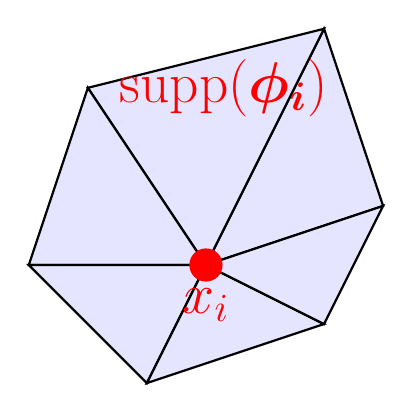
\begin{tikzpicture}[scale=1.5]
            \draw[thick, fill=blue!10] (0,0) -- (1.5,0.5) -- (1,2) -- cycle;
            \draw[thick, fill=blue!10] (0,0) -- (1,2) -- (-1,1.5) -- cycle;
            \draw[thick, fill=blue!10] (0,0) -- (-1,1.5) -- (-1.5,0) -- cycle;
            \draw[thick, fill=blue!10] (0,0) -- (-1.5,0) -- (-0.5,-1) -- cycle;
            \draw[thick, fill=blue!10] (0,0) -- (-0.5,-1) -- (1,-0.5) -- cycle;
            \draw[thick, fill=blue!10] (0,0) -- (1,-0.5) -- (1.5,0.5) -- cycle;
            \fill[red] (0,0) circle (4pt) node [anchor=north, font=\huge, yshift=-5pt] {$x_i$};
            \node[font=\huge] at (0.15, 1.5) {\textcolor{red}{$\text{supp}(\boldsymbol{\phi_i})$}};
        \end{tikzpicture}
    \end{center}
\end{frame}

\section{The Reference Element}

\begin{frame}{Barycentric Coordinates and the Master Element}
    To compute integrals efficiently, we map every  element $K_e$ to a reference one $\hat{K}$.
    
    For a 2D simplex, $\hat{K}$ is the unit triangle. Local shape functions:
    
    $$ \hat{\phi}_0(\xi_1, \xi_2) = 1 - \xi_1 - \xi_2, \quad \hat{\phi}_1(\xi_1, \xi_2) = \xi_1, \quad \hat{\phi}_2(\xi_1, \xi_2) = \xi_2 $$
   .
    
    \begin{center}
    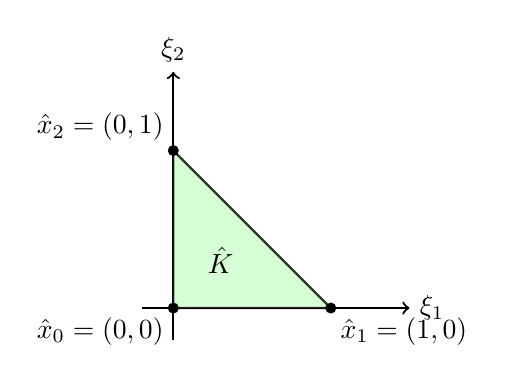
\begin{tikzpicture}[scale=2]
        \draw[->, thick] (-0.2,0) -- (1.5,0) node[right] {$\xi_1$};
        \draw[->, thick] (0,-0.2) -- (0,1.5) node[above] {$\xi_2$};
        \draw[thick, fill=green!20, opacity=0.8] (0,0) -- (1,0) -- (0,1) -- cycle;
        \fill (0,0) circle (1pt) node[below left] {$\hat{x}_0 = (0,0)$};
        \fill (1,0) circle (1pt) node[below right] {$\hat{x}_1 = (1,0)$};
        \fill (0,1) circle (1pt) node[above left] {$\hat{x}_2 = (0,1)$};
        \node at (0.3, 0.3) {$\hat{K}$};
    \end{tikzpicture}
    \end{center}
\end{frame}

\begin{frame}{Mapping and Quadrature}
    The physical coordinates $x \in K_e$ are obtained via the mapping $x:\hat K \to K_e$:
    $$ x(\bm{\xi}) = \sum_{a=1}^{N_{nodes}} x_a^e \hat{\phi}_a(\bm{\xi})\in \R^2 \quad\Rightarrow\quad \frac{\partial \bm{x}}{\partial \bm{\xi}} = [(x_1^e - x_3^e) \, (x_2^3 - x_3^e)] \in \R^{2\times 2}$$
    
    Let $J = \frac{\partial x}{\partial \xi}$ be the Jacobian of the transformation. To compute integrals in FE:
    \begin{enumerate}
        \item  $$ \int_{K_e} \psi(x) \, dx = \int_{\hat{K}} \psi(x(\bm{\xi})) |\det J (\bm{\xi})| \, d\hat{\Omega} $$
    
        \item Gradients are transformed using the inverse transpose Jacobian:
    $$ \nabla_x \phi_a^e = \frac{\partial \phi_a^e}{x_i} = \frac{\partial \phi_a^e}{\partial \xi_j}\frac{\partial \xi_j}{\partial x_i} =  J^{-T}(\bm{\xi}) \nabla_\xi \hat{\phi}_a(\bm{\xi}) $$
        \item The  integrals $\int_{\hat{K}} (\dots) d\hat{\Omega}$ are evaluated using numerical quadrature  on $\hat{K}$.
            $$ \int_{\hat{K}} \psi(x(\xi)) | \det J | d\hat{\Omega} \approx \sum_q \psi(x(\xi_q)) | \det J(\xi_q) | w_q $$
    \end{enumerate}
\end{frame}

\section{Assembly Arrays}
 
\begin{frame}{The FE Assembly Challenge}
    \textbf{Question:} How can one define the mappings required to efficiently manage the connectivity between element nodes and the global equation numbers?

    \begin{columns}
        \begin{column}{0.55\textwidth}
            \begin{center}
            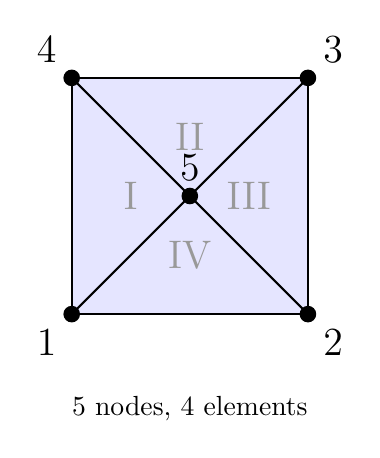
\begin{tikzpicture}[scale=3.0]
                \draw[thick, fill=blue!10] (0,0) rectangle (1,1);
                \draw[thick] (0,0) -- (1,1);
                \draw[thick] (0,1) -- (1,0);

                % Node labels (large font)
                \fill (0,0) circle (1pt) node[below left=2pt, font=\Large] {1};
                \fill (1,0) circle (1pt) node[below right=2pt, font=\Large] {2};
                \fill (1,1) circle (1pt) node[above right=2pt, font=\Large] {3};
                \fill (0,1) circle (1pt) node[above left=2pt, font=\Large] {4};
                \fill (0.5,0.5) circle (1pt) node[above=2pt, font=\Large] {5};
        
                % Element labels
                \node[font=\Large, gray!80] at (0.25, 0.5) {I};
                \node[font=\Large, gray!80] at (0.5, 0.75) {II};
                \node[font=\Large, gray!80] at (0.75, 0.5) {III};
                \node[font=\Large, gray!80] at (0.5, 0.25) {IV};
        
                % Annotations
                \node at (0.5, -0.4) {5 nodes, 4 elements};
            \end{tikzpicture}
            \end{center}
        \end{column}
        \begin{column}{0.4\textwidth}
            \begin{itemize}
                \item Element \phantom{II}I: $1\quad 4\quad 5$
                \item Element \phantom{I}II: $4\quad 5 \quad 3$
                \item Element III: $5\quad 2 \quad 3$
                \item Element IV: $1\quad 2 \quad 5$
            \end{itemize}
            
            \vspace{0.5cm}
        $$ K_{55} = \int_{K_I\cup K_{II} \cup K_{III} \cup K_{IV}} (\dots)\,dx $$
        \end{column}
    \end{columns}
\end{frame}

\begin{frame}{Connectivity and Equation Numbering}
    Assembly maps local element contributions $k^e_{ab}$ and $f^e_a$ to the global matrices $K_{ij}$ and $F_i$.
    
    \vspace{0.3cm}
    \textbf{1. The Element Node Matrix (IEN):}
    $$ \text{IEN}[e, a] \in \mathbb{N} $$
    Maps local node $a \in \{1, \dots, n_{dof}\}$ of element $e \in \{1, \dots, N_{el}\}$ to its \textbf{global node index}.
    
    \vspace{0.3cm}
    \textbf{2. The Destination Array (ID):}
    $$ \text{ID}[i] \in \mathbb{Z} $$
    Maps global node index $i$ to its \textbf{global DoF}\footnote{DoF: Degree of Freedom. Dirichlet nodes are set to -1}. 

    \textbf{3. The Location Matrix (LM):}
    $$ \text{LM}[e, a] \coloneqq ID[IEN[e,a] $$
    Maps local node $a$ in element $e$ to its global DoF.

\end{frame}

\begin{frame}{Assembly algorithm}

    \begin{itemize}
        \item For each element $K_e$:
            \begin{itemize}
                \item For each local nodes $a,b$:
                    \begin{itemize}
                            \item Update local contributions to global matrix
                    \end{itemize}
            \end{itemize}
    \end{itemize}
    $$ K_{ij} \leftarrow K_{ij} + k^e_{ab} $$
    where $i = LM[e,a], j = LM[e,j]$. 
\end{frame}

\section{Minimal Example}

\begin{frame}{Example: Geometry and IEN Matrix}
    Consider a square domain partitioned into 2 elements ($N_{el}=2$) with 4 global nodes ($N_{nodes}=4$). Dirichlet BCs in left boundary.
    
    \begin{columns}
        \begin{column}{0.4\textwidth}
            \begin{center}
            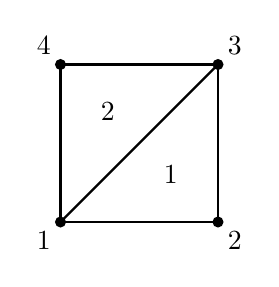
\begin{tikzpicture}[scale=2]
                \draw[thick] (0,0) rectangle (1,1);
                \draw[thick] (0,0) -- (1,1);
                
                \fill (0,0) circle (1pt) node[below left] {1};
                \fill (1,0) circle (1pt) node[below right] {2};
                \fill (1,1) circle (1pt) node[above right] {3};
                \fill (0,1) circle (1pt) node[above left] {4};
                
                \node at (0.7, 0.3) {1};
                \node at (0.3, 0.7) {2};
            \end{tikzpicture}
            \end{center}
        \end{column}
        \begin{column}{0.6\textwidth}
            \only<1>{
                \textbf{Element Node Matrix (IEN):}
                \vspace{0.2cm}
                
                \renewcommand{\arraystretch}{1.5}
                \begin{tabular}{|c|c|c|c|}
                    \hline
                    Element ($e$) & $a=1$ & $a=2$ & $a=3$ \\ \hline
                    1 & 1 & 2 & 3 \\ \hline
                    2 & 1 & 3 & 4 \\ \hline
                \end{tabular}
                \vspace{0.2cm}
                
                $\text{IEN}[1, :] = [1, 2, 3]$ \\
                $\text{IEN}[2, :] = [1, 3, 4]$
            }
            \only<2>{
                \textbf{Destination Array (ID):}
                \renewcommand{\arraystretch}{1.2}
                \begin{table}[]
                    \centering
                    \begin{tabular}{|c|c|c|c|c|}
                        \hline
                        Global Node ($i$) & 1 (BC) & 2  & 3  & 4 (BC) \\ \hline
                        $\text{ID}[i]$ & 0 & 1 & 2 & 0 \\ \hline
                    \end{tabular}
                \end{table}
            }
            \only<3>{
                \textbf{Location Matrix (LM):} $\text{LM}[e, a] = \text{ID}[\text{IEN}[e, a]]$
                \renewcommand{\arraystretch}{1.5}
                \begin{table}[]
                    \centering
                    \begin{tabular}{|c|c|c|c|}
                        \hline
                        Element ($e$) & $a=1$ & $a=2$ & $a=3$ \\ \hline
                        1 & $\text{ID}[1] = 0$ & $\text{ID}[2] = 1$ & $\text{ID}[3] = 2$ \\ \hline
                        2 & $\text{ID}[1] = 0$ & $\text{ID}[3] = 2$ & $\text{ID}[4] = 0$ \\ \hline
                    \end{tabular}
                \end{table}
    
                Element II only contributes to global equation 2!

            }
        \end{column}
    \end{columns}
\end{frame}

\begin{frame}[fragile]{The Assembly Loop}
    \begin{footnotesize}
    \begin{algorithmic}[1]
    \State Initialize $K = \mathbf{0}$, $F = \mathbf{0}$
    \For{$e = 1 \dots N_{el}$}
        \State Compute $k^e \in \mathbb{R}^{3 \times 3}$, $f^e \in \mathbb{R}^3$ via reference element quadrature
        \For{$a = 1 \dots 3$}
            \State $i = \text{LM}[e, a]$
            \If{$i > 0$} \Comment{Free node}
                \State $F_i \leftarrow F_i + f^e_a$
                \For{$b = 1 \dots 3$}
                    \State $j = \text{LM}[e, b]$
                    \If{$j > 0$} \Comment{Free node interaction}
                        \State $K_{ij} \leftarrow K_{ij} + k^e_{ab}$
                    \Else \Comment{Dirichlet boundary interaction}
                        \State $F_i \leftarrow F_i - k^e_{ab} \, g_D(\text{node } \text{IEN}[e,b])$
                    \EndIf
                \EndFor
            \EndIf
        \EndFor
    \EndFor
    \end{algorithmic}
    \end{footnotesize}
\end{frame}

\end{document}
